\flushleft
\textbf{Conceptual Framework of the Study}\\

\justifying
\parx
The conceptual framework (refer to Figure \ref{fig:conceptual_framework}) represents the relationship
and flow of the concept of developing a visual programming software for learning the
fundamentals of programming.

\parx
It shows the order of actions required by the study to achieve the desired
output following the design of the context diagram (refer to Figure \ref{fig:context_diagram})

\parx
The inputs has the following requirements for the development of the study.
Knowledge requirements include programming, programming languages, parsing,
evaluation, C++ programming language, user-interface design, user-experience
design, data flow diagram, and context diagram.  Software requirement include
Linux 5.4 - Manjaro as operating system and distribution, Vim as text and code
editor, terminal, Kha and zui library for graphics, and the C++ programming
language for development. Microsoft Windows 7 and above, C++ Runtime libraries,
and the C++ programming language for deployment.  Hardware requirement are
machine with at at least Intel Core 2 Duo at 1.4 GHz, 2 GB of RAM, and 80 GB
HDD storage for development. At least Intel Core 2 Duo at 1.4 GHz, 2 GB of RAM,
and at least 1 GB HDD storage space for deployment.

\parx
The process to be followed and used for the development of the software is the V model.
The process model involves the requirements of gathering necessary data and information
from respondents through conducted survey. High-level design of the implementation of
the requirements of its technical usage for system design. Design of the relationships
and dependencies of the modules, creation of diagrams, and selection of technology to
be used. Preparation of the design and test method for each module. Followed by the
coding of the modules and the software. The evaluation is based on the ISO/IEC/IEEE
29119-4.2015, specifically the experience-based test design technique, to assure the
functionality, efficiency, usability, portability, and reliability of the software.

\parx
The impact expected from the study is the availability of a software designed for
learning to program and its fundamentals for learners, students, and educators.
Another impact is the improvements in the understanding, skills, and academic
performances of the students in the course of programming.

\begin{figure}[H]
	\centering
	\captionsetup{justification=centering}
	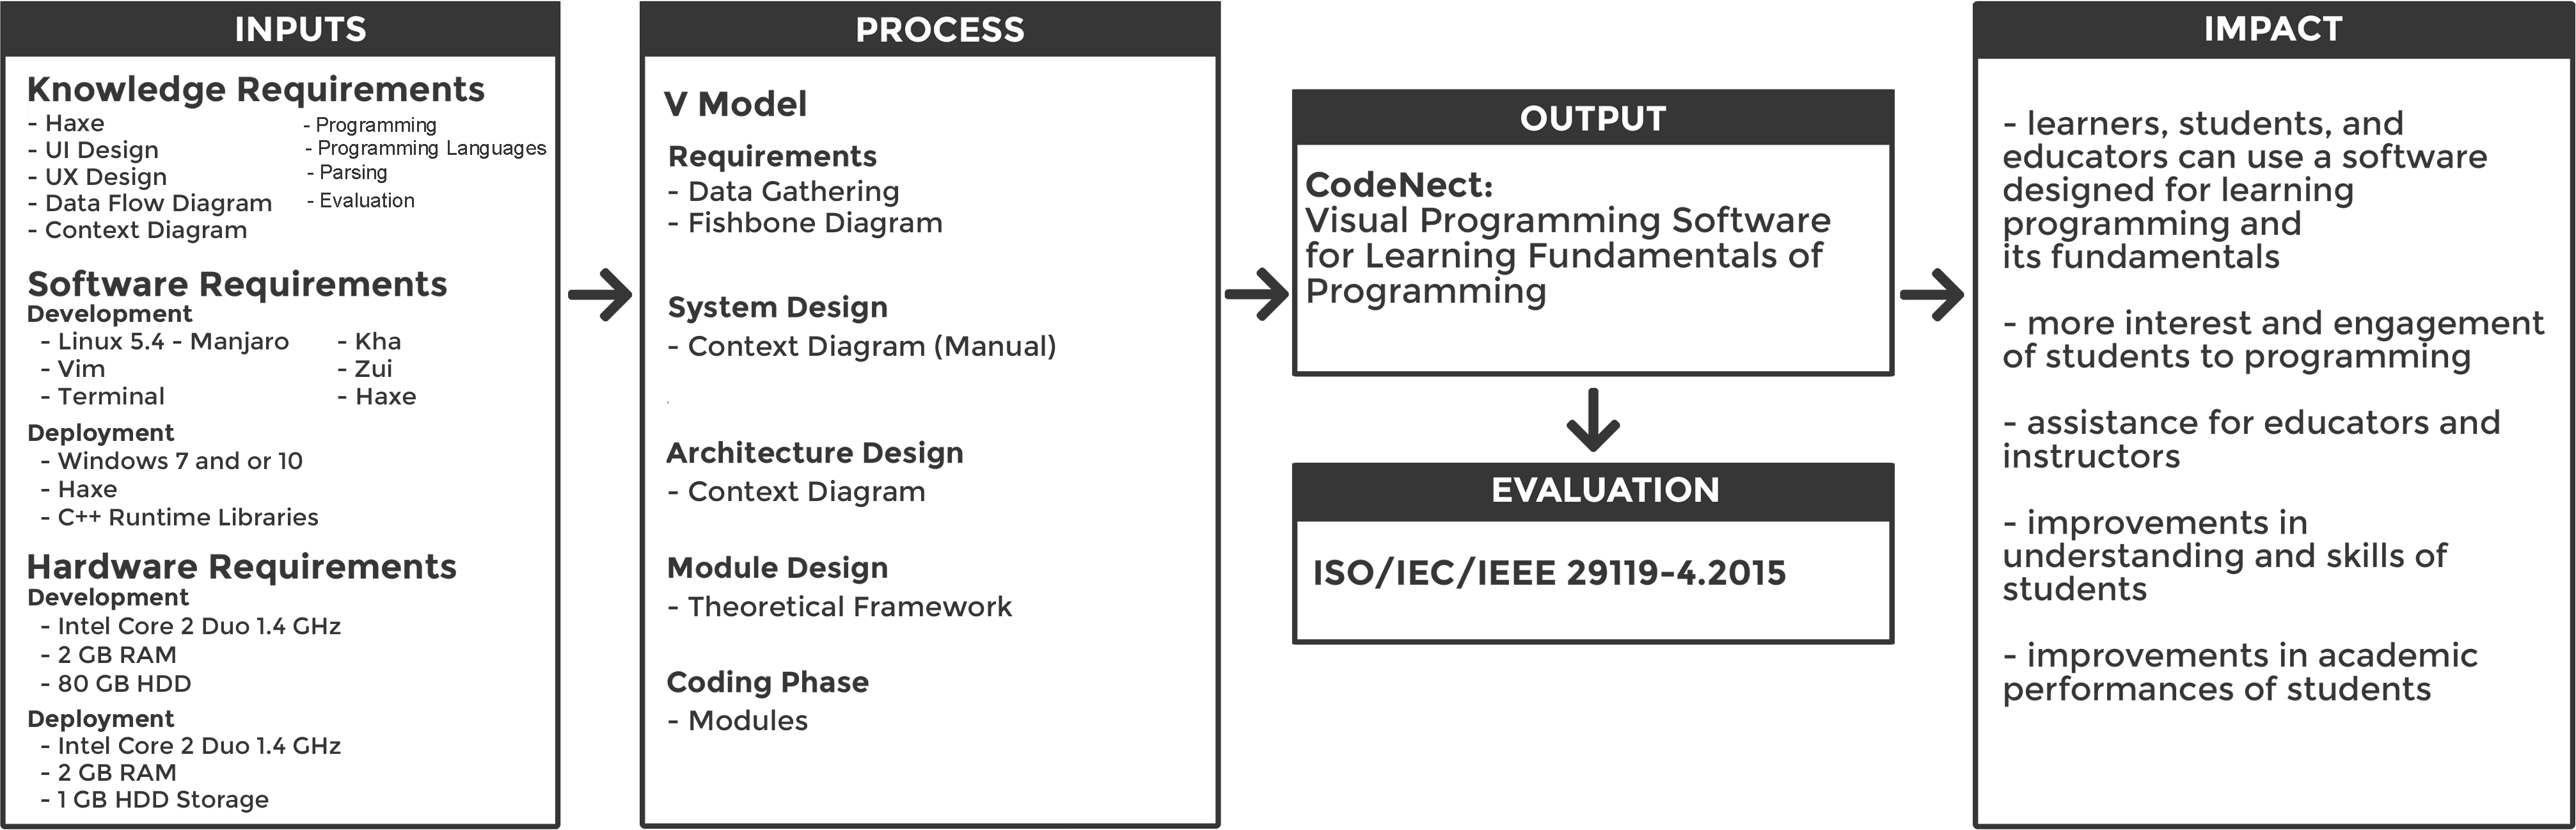
\includegraphics[width=\linewidth]{figures/conceptual_framework.png}
	\caption[Conceptual Framework]{Conceptual Framework of proposed CodeNect: Visual Programming Software for Learning Fundamentals of Programming}
	\label{fig:conceptual_framework}
\end{figure}
